\documentclass[12pt,a4paper]{article}

\usepackage{fontspec}
\XeTeXlinebreaklocale "th"
\XeTeXlinebreakskip = 0pt plus 1pt
\defaultfontfeatures{Ligatures=TeX}
\setmainfont[
  Path={fonts/TH Sarabun PSK V-1/},
  Extension=.ttf,
  UprightFont={*},
  BoldFont={* Bold},
  ItalicFont={* Italic},
  BoldItalicFont={* BoldItalic}
]{THSarabun}
\setmonofont{Latin Modern Mono}

\usepackage{graphicx}
\usepackage{textcomp}
\usepackage{amsmath,amssymb,float,caption,subcaption,xcolor,hyperref,fancyhdr,tikz}
\usetikzlibrary{positioning,arrows.meta,calc}
\usepackage{geometry,booktabs,array,tabularx}
\geometry{margin=1in}
\setlength{\headheight}{14.5pt}
\pagestyle{fancy}\fancyhf{}\lhead{IBR Grid-Following / Grid-Forming: State Order และ Small-Signal Stability}\rhead{\thepage}
\hypersetup{colorlinks=true,linkcolor=blue,urlcolor=blue,citecolor=blue}
\renewcommand{\arraystretch}{1.12}
\captionsetup[table]{skip=7pt}
\emergencystretch=2em
\linespread{1.15}

\renewcommand{\abstractname}{บทคัดย่อ}
\renewcommand{\contentsname}{สารบัญ}
\renewcommand{\figurename}{รูปที่}
\renewcommand{\tablename}{ตารางที่}
\renewcommand{\refname}{เอกสารอ้างอิง}

\title{\textbf{แบบจำลอง Inverter-Based Resource (IBR) แบบลดรูป 6 states: Grid-Following และ Grid-Forming}\\
\large State Order, Small-Signal Stability (SSSA) และการเปรียบเทียบ $i_d/i_q/P/Q$ บน SMIB}
\date{22 กรกฎาคม 2569}

\begin{document}
\maketitle

\begin{abstract}
รายงานฉบับนี้อธิบาย \emph{ลำดับ state (state order)} ของแบบจำลอง IBR แบบลดรูป \textbf{2 ชุด ชุดละ
6 states} ที่พัฒนาเป็น project-owned MATLAB code ตามโครงสร้างของงาน EECON49 และเชื่อมต่อกับ ideal
infinite bus ผ่าน $Z_{line}$ (single-machine infinite-bus, SMIB) ได้แก่ (i) \textbf{Grid-Following
(GFL) 6 states} และ (ii) \textbf{Grid-Forming VSG (GFM) 6 states} โดยแต่ละชุดจัดเป็น \emph{3 บล็อก
บล็อกละ 2 states}: ฝั่ง GFL = IBR + GFL(PLL) + PQ ส่วนฝั่ง GFM = IBR + VSG + GFM รายงานนำเสนอเฉพาะผล
\textbf{Small-Signal Stability (SSSA)} คือ eigenvalue spectrum พร้อมกราฟ real/imag บนระนาบเชิงซ้อน
กราฟความถี่โมดัล (Hz) และผล $i_d,i_q,P,Q$ ทั้งค่า equilibrium และ time-domain ring-down โดย
\emph{ไม่} แสดงผล power flow ตามที่กำหนด ทั้งสองแบบจำลอง \emph{มีโหมดสั่น (complex mode)} ตามที่คาดไว้ในทฤษฎี:
GFL มีโหมด PLL ที่ $\sim0.34$ Hz และ GFM มีโหมด swing ที่ $\sim10.8$ Hz สมการทุกตัวมีที่มาอ้างอิงได้
และไม่มีการปรับพารามิเตอร์เพื่อให้ผลตรงกับค่าใด ๆ
\end{abstract}
\newpage
\tableofcontents
\newpage

\section{ขอบเขตและ Source Discipline}

รายงานนี้เน้นโครงสร้าง state และผล SSSA ของ IBR แบบลดรูป 6 states ไม่ครอบคลุมการ verify power flow
(ตามที่ผู้ใช้กำหนดให้งดแสดง PF) โครงสร้างและค่าพารามิเตอร์ยึดตามสูตรของงาน EECON49-P4~\cite{eecon49}
สมการย่อยของแต่ละบล็อกสืบสาวได้จากแหล่งอ้างอิงมาตรฐาน:

\begin{itemize}
  \item \textbf{GFL 6 states.} วง current control และ SRF-PLL เป็น \texttt{SOURCE\_DEFINED} ที่สืบจาก
  Yazdani \& Iravani~\cite{yazdani2010} และ Teodorescu et al.~\cite{teodorescu2011}; ลูปกำลัง PQ ชั้นนอก
  เป็น \texttt{APPROVED\_PROJECT\_DERIVED} ตาม Bacha et al.~\cite{bacha2014}
  \item \textbf{GFM 6 states.} virtual swing (VSG) และการสร้างแรงดันแบบ Q-V droop สืบจากแนวทาง VSG
  (Pogaku et al.~\cite{pogaku2007}, Sakimoto et al.~\cite{sakimoto2015}); การประกอบเป็นแบบลดรูป 6 states
  เป็น \texttt{PROJECT\_DERIVED\_SOURCE\_MAPPED}
\end{itemize}

การลดรูปเป็น 6 states (เทียบกับแบบจำลองเต็มอันดับสูง): ตัดตัวกรองวัดกำลัง/แรงดัน, ตัด integrator ของ
current loop (เหลือ proportional + decoupling), และคงไว้เฉพาะพลวัตหลักของแต่ละบล็อก จุดจำแนกและค่าเกน
freeze ไว้ที่ \texttt{docs/project/IBR\_REDUCED6\_EECON49\_MANIFEST.md}

ทั้งสองแบบจำลองรันบน 100-MVA base ที่จุดทำงานเดียวกัน: terminal voltage $V=1.0\angle0^\circ$ pu,
$P=0.40$ pu, $Q=0.10$ pu, สายส่งสู่ infinite bus $Z_{line}=0.02+j0.20$ pu ค่า SSSA ทั้งหมดได้จาก
in-house Schur-complement linearisation รอบ equilibrium ที่ตรวจแล้วว่า residual อยู่ระดับ machine precision

\section{คำอธิบายแบบจำลองและลำดับ State}

DAE แบบ input-driven ที่ใช้ร่วมกันทั้ง equilibrium, SSSA และ time-domain simulation คือ
\begin{equation}
\dot x = f(x,y,u),\qquad 0 = g(x,y,u),
\label{eq:dae}
\end{equation}
โดย $x$ คือ device differential states, $y=[\Re(V)\ \Im(V)]^T$ คือ algebraic bus voltage และ
$u=[P_{ref}\ Q_{ref}]^T$ คือ input references ปริมาณ device ทำงานบน inverter base ส่วน current injection
และ electrical power คืนค่าบน system base ($\kappa=S_{base}/M_{base}$) กรอบ dq ใช้
$V_{dq}=Ve^{-j\delta}$ โดย $v_d=\Re$, $v_q=\Im$ และ current injection
$I_{net}=(i_d+ji_q)e^{j\delta}/\kappa$

\subsection{แบบจำลอง Grid-Following (GFL) 6 states}
\label{subsec:gfl}

GFL \emph{ติดตาม} แรงดันกริด: ใช้ SRF-PLL จับมุมกริดเพื่อสร้างกรอบ $dq$ แล้วสังเคราะห์กระแสให้กำลังจริง/
รีแอกทีฟตามคำสั่ง $P_{ref}/Q_{ref}$ โครงสร้างแบ่งเป็นสามบล็อก บล็อกละ 2 states:

\begin{equation}
\dot x_{\text{GFL}} =\Big[\,
\underbrace{\dot i_d,\ \dot i_q}_{\text{IBR: current + L-filter}},\ \,
\underbrace{\dot\delta_{PLL},\ \dot\xi_{PLL}}_{\text{GFL: PLL synchronisation}},\ \,
\underbrace{\dot\xi_{P},\ \dot\xi_{Q}}_{\text{PQ: outer power loop}}
\,\Big]^{T}= f(x_{\text{GFL}},y,u).
\label{eq:gfl-order}
\end{equation}

\begin{table}[H]\centering\small
\caption{ลำดับ state ของ GFL 6-state}
\label{tab:order-gfl}
\begin{tabular}{clll}\toprule
\# & State & บล็อก & ความหมาย\\\midrule
1 & $i_d$        & IBR & กระแสแกน $d$ ของ L-filter (inverter base)\\
2 & $i_q$        & IBR & กระแสแกน $q$ ของ L-filter (inverter base)\\
3 & $\delta_{PLL}$ & GFL & มุมของ SRF-PLL (rad)\\
4 & $\xi_{PLL}$  & GFL & integrator ของ PLL PI (pu$\cdot$s)\\
5 & $\xi_{P}$    & PQ  & integrator ลูปกำลังจริงชั้นนอก\\
6 & $\xi_{Q}$    & PQ  & integrator ลูปกำลังรีแอกทีฟชั้นนอก\\\bottomrule
\end{tabular}\end{table}

\noindent\textbf{คำอธิบายแต่ละ state (สำหรับผู้ไม่มีพื้นฐาน).}
\begin{itemize}
  \item \textbf{$i_d,i_q$ (กระแสจริงที่ไหลออก).} กระแสที่อินเวอร์เตอร์ฉีดออกจริงในกรอบหมุน: $i_d$ สัมพันธ์กับ
  กำลังจริง ($P$), $i_q$ สัมพันธ์กับกำลังรีแอกทีฟ ($Q$) เป็นผลลัพธ์ของฮาร์ดแวร์ + ตัวกรอง L
  \item \textbf{$\delta_{PLL}$ (มุมของ PLL).} มุมที่ PLL ประมาณได้ ใช้เป็นแกนอ้างอิง $dq$; GFL \emph{ต้อง}
  รู้มุมกริดก่อนจึงฉีดกระแสให้ตรงเฟสได้ (ต่างจาก GFM ที่ไม่มี PLL)
  \item \textbf{$\xi_{PLL}$ (ตัวสะสมของ PLL).} หน่วยความจำสะสมของ PI ใน PLL บังคับให้มุมล็อกกับกริด
  ($v_q\to0$) เป็นตัวสร้าง \emph{โหมดสั่นของ PLL}
  \item \textbf{$\xi_{P},\xi_{Q}$ (ตัวสะสมลูปกำลังชั้นนอก).} ปรับคำสั่งกระแส $i_d^{ref},i_q^{ref}$ จนกำลัง
  ที่จ่ายออกเท่ากับ $P_{ref}/Q_{ref}$ พอดี (ขจัด steady-state error)
\end{itemize}

\noindent สมการ governing แยกตามบล็อก \emph{พร้อมแหล่งที่มา}:

\noindent\textbf{บล็อก GFL --- PLL synchronisation} (\texttt{SOURCE\_DEFINED}: Teodorescu~\cite{teodorescu2011}
eq.~4.38 รูป ODE; Yazdani~\cite{yazdani2010} eq.~8.1)\textbf{.} \emph{ทำหน้าที่:} จับมุมกริด
\begin{align}
v_d &= \Re(Ve^{-j\delta_{PLL}}),\quad v_q = \Im(Ve^{-j\delta_{PLL}}),\\
\dot\xi_{PLL} &= v_q,\qquad
\dot\delta_{PLL} = k_{p,PLL}\,v_q + k_{i,PLL}\,\xi_{PLL}.
\label{eq:gfl-pll}
\end{align}
สังเกตว่า PI output คือความถี่ (rad/s) ที่บวกเข้า $\omega_0$ โดยตรง \emph{ไม่มีตัวคูณ $\omega_b$} ด้วยเกน
$k_{p,PLL}=1.20,\ k_{i,PLL}=5.00$ (EECON49) ลูป PLL อันดับสองมี $\zeta<1$ จึงให้ \emph{คู่ complex}
(โหมดซิงโครไนซ์ที่สั่นได้)

\noindent\textbf{บล็อก PQ --- outer power loop} (\texttt{APPROVED\_PROJECT\_DERIVED}: Bacha~\cite{bacha2014})\textbf{.}
\emph{ทำหน้าที่:} คุมกำลังให้ตรงคำสั่ง (วัดกำลังแบบพีชคณิต ไม่มีตัวกรอง)
\begin{align}
P &= \Re(V\overline{I_{net}}),\quad Q = \Im(V\overline{I_{net}}),\\
\dot\xi_{P} &= P_{ref}-P,\qquad \dot\xi_{Q} = Q_{ref}-Q,\\
i_d^{ref} &= k_{pP}(P_{ref}-P)+k_{iP}\xi_{P},\quad
i_q^{ref} = -\big(k_{pQ}(Q_{ref}-Q)+k_{iQ}\xi_{Q}\big).
\end{align}

\noindent\textbf{บล็อก IBR --- current + L-filter} (\texttt{SOURCE\_DEFINED}: Yazdani~\cite{yazdani2010}
eq.~8.45--8.50; ลดรูปเป็น proportional)\textbf{.} \emph{ทำหน้าที่:} บังคับกระแสจริงให้ตามคำสั่งด้วย
current control แบบ proportional + decoupling บน plant ของ L-filter
\begin{align}
v_{td} &= k_{pi}(i_d^{ref}-i_d)+R_t i_d-\omega_{PLL}L\,i_q+v_d,\\
\tfrac{L}{\omega_b}\dot i_d &= \omega_{PLL}L\,i_q-R_t i_d+v_{td}-v_d
\;=\; k_{pi}(i_d^{ref}-i_d),
\end{align}
(แกน $q$ สมมาตร) เนื่องจาก decoupling ตัดพจน์ไขว้ ลูปกระแสจึงเป็นอันดับหนึ่ง (โหมดจริงที่เร็ว)

\subsection{แบบจำลอง Grid-Forming (GFM) 6 states}
\label{subsec:gfm}

GFM \emph{สร้าง} แรงดันและความถี่เอง โดยใช้โครงสร้าง Virtual Synchronous Generator (VSG): สมการ swing
กำหนดมุมโรเตอร์ (synchronizing power) \emph{โดยไม่มี PLL} และ Q-V droop กำหนดขนาดแรงดันภายใน โครงสร้าง
สามบล็อก บล็อกละ 2 states:

\begin{equation}
\dot x_{\text{GFM}} =\Big[\,
\underbrace{\dot i_d,\ \dot i_q}_{\text{IBR: current + L-filter}},\ \,
\underbrace{\dot\omega,\ \dot\delta}_{\text{VSG: virtual swing}},\ \,
\underbrace{\dot E,\ \dot\xi_{V}}_{\text{GFM: voltage forming}}
\,\Big]^{T}= f(x_{\text{GFM}},y,u).
\label{eq:gfm-order}
\end{equation}

\begin{table}[H]\centering\small
\caption{ลำดับ state ของ GFM 6-state}
\label{tab:order-gfm}
\begin{tabular}{clll}\toprule
\# & State & บล็อก & ความหมาย\\\midrule
1 & $i_d$    & IBR & กระแสแกน $d$ ของ L-filter (inverter base)\\
2 & $i_q$    & IBR & กระแสแกน $q$ ของ L-filter (inverter base)\\
3 & $\omega$ & VSG & ความเร็วโรเตอร์เสมือน (pu)\\
4 & $\delta$ & VSG & มุมโรเตอร์เทียบกริด / load angle (rad)\\
5 & $E$      & GFM & ขนาดแรงดันภายใน (Q-V droop)\\
6 & $\xi_{V}$& GFM & integrator ของ voltage PI (แกน $d$)\\\bottomrule
\end{tabular}\end{table}

\noindent\textbf{คำอธิบายแต่ละ state (สำหรับผู้ไม่มีพื้นฐาน).}
\begin{itemize}
  \item \textbf{$i_d,i_q$.} เช่นเดียวกับ GFL แต่กระแสถูกสั่งจากลูปแรงดัน (voltage-forming) ไม่ใช่ลูปกำลัง
  \item \textbf{$\omega$ (ความเร็วโรเตอร์เสมือน).} อินเวอร์เตอร์ ``แกล้ง'' เป็นเครื่องจักรหมุนที่มีความเฉื่อย
  (virtual inertia) เมื่อกำลังเข้า/ออกไม่สมดุล ความเร็วจะเปลี่ยน คือหัวใจของพฤติกรรมหน่วงคล้ายเครื่องจริง
  \item \textbf{$\delta$ (มุมโรเตอร์ / load angle).} มุมที่โรเตอร์เสมือนนำหน้ากริด เป็นตัวกำหนดการไหลของกำลังจริง
  และเป็นกลไก \emph{synchronizing power} ที่ดึงเครื่องให้ซิงค์โดยไม่ต้องมี PLL เป็นตัวสร้าง \emph{โหมด swing}
  \item \textbf{$E$ (ขนาดแรงดันภายใน).} แรงดันที่ VSG สร้างขึ้น ปรับตาม Q-V droop เพื่อคุมกำลังรีแอกทีฟ/แรงดัน
  \item \textbf{$\xi_{V}$ (ตัวสะสมของ voltage loop).} หน่วยความจำสะสมของ PI แรงดัน ทำให้แรงดันปลายทางตามค่า $E$
\end{itemize}

\noindent สมการ governing แยกตามบล็อก \emph{พร้อมแหล่งที่มา}:

\noindent\textbf{บล็อก VSG --- virtual swing (ไม่มี PLL)} (\texttt{SOURCE\_DEFINED/VSG}:
Pogaku~\cite{pogaku2007}, Sakimoto~\cite{sakimoto2015})\textbf{.} \emph{ทำหน้าที่:} สร้างมุม/ความถี่จาก
สมดุลกำลัง
\begin{equation}
\dot\omega = \frac{P_{ref}-P-D_v(\omega-1)}{M},\qquad
\dot\delta = \omega_b(\omega-1).
\label{eq:gfm-swing}
\end{equation}
ด้วย $M=0.08$ s (ความเฉื่อยต่ำ) และ $D_v=1.50$ ลูป swing มี $\zeta<1$ จึงให้ \emph{คู่ complex}
(โหมด electromechanical ที่สั่น)

\noindent\textbf{บล็อก GFM --- voltage forming (Q-V droop + voltage PI)} (\texttt{PROJECT\_DERIVED\_SOURCE\_MAPPED})\textbf{.}
\emph{ทำหน้าที่:} กำหนดขนาดแรงดัน บนสายที่เด่นด้วยรีแอกแตนซ์ ($v_{gd}=E+Xi_q$, $v_{gq}=-Xi_d$) จึงต้องจับคู่
\emph{ไขว้แกน}: แรงดันแกน $d$ คุมด้วยกระแส $q$ (reactive) และแกน $q$ คุมด้วยกระแส $d$ (active/synchronizing)
\begin{align}
\dot E &= \big(k_Q(Q_{ref}-Q)-k_E(E-|V|)\big)/\tau_E,\qquad \dot\xi_{V}=E-v_{gd},\\
i_q^{ref} &= -\big(k_{pV}(E-v_{gd})+k_{iV}\xi_{V}\big),\qquad
i_d^{ref} = k_{pV}(0-v_{gq}).
\end{align}
(การจับคู่แบบตรงแกนถูกตรวจแล้วว่า \emph{ไม่เสถียร}; การจับคู่ไขว้นี้เสถียร)

\noindent\textbf{บล็อก IBR --- current + L-filter.} เหมือน GFL (proportional + decoupling) แต่กรอบหมุนใช้
มุมโรเตอร์ $\delta$ จาก swing (ไม่ใช่ $\delta_{PLL}$)

\section{Small-Signal Stability (SSSA)}

เมื่อ linearise ระบบพลวัตรอบจุดทำงาน จะเขียนได้ในรูป state-space มาตรฐาน
\begin{equation}
\Delta\dot x = A\,\Delta x + B\,\Delta u,
\label{eq:axbu}
\end{equation}
โดย $A$ คือ \emph{system (state) matrix} ที่กำหนดพลวัตภายในและเสถียรภาพเชิงเล็ก ส่วน $B$ คือ
\emph{input matrix} ที่เชื่อมสัญญาณควบคุมภายนอก $\Delta u$ แบบจำลองทั้งสองในรายงานนี้ \textbf{ไม่มี
AVR/PSS} จึงไม่มีสัญญาณควบคุมภายนอกที่จะปรับ ($\Delta u=0$) สมการ~\eqref{eq:axbu} จึงลดเหลือ
$\Delta\dot x=A\,\Delta x$ การวิเคราะห์ SSSA จึงพิจารณาเฉพาะ eigenvalue ของ $A$ เท่านั้น เมทริกซ์ $A$
ได้จากการ linearise DAE ใน~\eqref{eq:dae} เชิงตัวเลข (central difference, $h=10^{-6}$) รอบ equilibrium
แล้ว eliminate algebraic voltage ด้วย Schur complement
\begin{equation}
A = J_{xx}-J_{xy}J_{yy}^{-1}J_{yx},\qquad \Delta\dot x = A\,\Delta x,
\end{equation}
จากนั้นหา eigenvalue $\lambda_i=\sigma_i+j\omega_{d,i}$ พร้อม $f_i=|\omega_{d,i}|/2\pi$ และ
$\zeta_i=-\sigma_i/|\lambda_i|$ โหมดจะ asymptotically stable เมื่อ $\sigma_i<0$

ตารางที่~\ref{tab:A-gfl} และ~\ref{tab:A-gfm} แสดง \emph{เมทริกซ์ $A$ จริง} (ขนาด $6\times6$) ของทั้งสอง
แบบจำลอง โดยหัวแถว/หัวคอลัมน์คือ state ตามลำดับใน~\eqref{eq:gfl-order} และ~\eqref{eq:gfm-order} ($B=0$
จึงมีเฉพาะ $A$) สังเกตว่าแถว $\dot\delta_{PLL}=\omega_b(\omega-1)$ ของ GFM ให้ค่า $A(\delta,\omega)=\omega_b=377$
และแถว current loop มีค่าขนาดใหญ่ (โหมดเร็ว) ส่วนช่อง $0$ คือไม่มีการเชื่อมโยงโดยตรง

\begin{table}[H]\centering\small
\caption{เมทริกซ์ $A$ ของ GFL 6-state ($\Delta\dot x = A\,\Delta x$, หน่วย 1/s)}
\label{tab:A-gfl}
\resizebox{\textwidth}{!}{\begin{tabular}{crrrrrr}\toprule
$A$ & $i_d$ & $i_q$ & $\delta_{PLL}$ & $\xi_{PLL}$ & $\xi_{P}$ & $\xi_{Q}$\\\midrule
$i_d$ & -1350 & +49.46 & -39.81 & 0 & +1885 & 0\\
$i_q$ & +49.46 & -1364 & -239.2 & 0 & 0 & -1885\\
$\delta_{PLL}$ & +0.24 & +0.024 & -1.166 & +5 & 0 & 0\\
$\xi_{PLL}$ & +0.2 & +0.02 & -0.972 & 0 & 0 & 0\\
$\xi_{P}$ & -0.988 & +0.082 & -0.066 & 0 & 0 & 0\\
$\xi_{Q}$ & -0.082 & +1.012 & +0.3966 & 0 & 0 & 0\\
\bottomrule
\end{tabular}
}
\end{table}

\begin{table}[H]\centering\small
\caption{เมทริกซ์ $A$ ของ GFM 6-state ($\Delta\dot x = A\,\Delta x$, หน่วย 1/s)}
\label{tab:A-gfm}
\resizebox{\textwidth}{!}{\begin{tabular}{crrrrrr}\toprule
$A$ & $i_d$ & $i_q$ & $\omega$ & $\delta$ & $E$ & $\xi_{V}$\\\midrule
$i_d$ & -934.9 & -18.1 & 0 & +819.8 & 0 & 0\\
$i_q$ & +18.1 & -934.9 & 0 & -326.1 & -904.8 & -3393\\
$\omega$ & -11.5 & +4.612 & -18.75 & -0.825 & 0 & 0\\
$\delta$ & 0 & 0 & +377 & 0 & 0 & 0\\
$E$ & -5.256 & -26.57 & 0 & -10.5 & -160 & 0\\
$\xi_{V}$ & -0.02 & +0.2 & 0 & +0.3604 & +1 & 0\\
\bottomrule
\end{tabular}
}
\end{table}

\subsection{Eigenvalue Spectrum}

ทั้งสองแบบจำลอง asymptotically stable ทุกโหมด (real part $<0$) โดย \textbf{GFL มีโหมด PLL สั่นที่}
$-0.58\pm j2.14$ ($f=0.34$ Hz, $\zeta=0.26$) และ \textbf{GFM มีโหมด swing สั่นที่} $-7.09\pm j67.6$
($f=10.76$ Hz, $\zeta=0.10$) นอกนั้นเป็นโหมดเร็ว (current loop) และโหมดจริง (PQ / voltage droop)

\begin{table}[H]\centering\small
\caption{Eigenvalue ของ GFL 6-state เรียงตาม real part จากมากไปน้อย พร้อมบทบาทของ dominant state}
\label{tab:eig-gfl}
\resizebox{\textwidth}{!}{\begin{tabular}{cl p{5.2cm} rrrr}\toprule
No & Dominant state & Role (what the state does) & Real (1/s) & Imag (1/s) & $f$ (Hz) & $\zeta$\\\midrule
01 & $\delta_{PLL}$ & SRF-PLL angle: synchronises the dq frame to the grid voltage & -5.821\,\texttimes\,10\textsuperscript{-1} & +2.145\,\texttimes\,10\textsuperscript{0} & 0.3414 & 0.2619\\
02 & $\delta_{PLL}$ & SRF-PLL angle: synchronises the dq frame to the grid voltage & -5.821\,\texttimes\,10\textsuperscript{-1} & -2.145\,\texttimes\,10\textsuperscript{0} & 0.3414 & 0.2619\\
03 & $\xi_{P}$ & outer active-power PI integrator (sets $i_d$ ref) & -1.356\,\texttimes\,10\textsuperscript{0} & 0 & 0.0000 & 1.0000\\
04 & $\xi_{Q}$ & outer reactive-power PI integrator (sets $i_q$ ref) & -1.435\,\texttimes\,10\textsuperscript{0} & 0 & 0.0000 & 1.0000\\
05 & $i_d$ & $d$-axis L-filter (converter) current & -1.306\,\texttimes\,10\textsuperscript{3} & 0 & 0.0000 & 1.0000\\
06 & $i_q$ & $q$-axis L-filter (converter) current & -1.406\,\texttimes\,10\textsuperscript{3} & 0 & 0.0000 & 1.0000\\
\bottomrule
\end{tabular}
}
\end{table}

\begin{table}[H]\centering\small
\caption{Eigenvalue ของ GFM 6-state เรียงตาม real part จากมากไปน้อย พร้อมบทบาทของ dominant state}
\label{tab:eig-gfm}
\resizebox{\textwidth}{!}{\begin{tabular}{cl p{5.2cm} rrrr}\toprule
No & Dominant state & Role (what the state does) & Real (1/s) & Imag (1/s) & $f$ (Hz) & $\zeta$\\\midrule
01 & $\xi_{V}$ & d-axis voltage-PI integrator (forms $|V|$) & -5.546\,\texttimes\,10\textsuperscript{-1} & 0 & 0.0000 & 1.0000\\
02 & $\delta$ & virtual load angle (swing angle vs grid) & -7.086\,\texttimes\,10\textsuperscript{0} & +6.763\,\texttimes\,10\textsuperscript{1} & 10.7639 & 0.1042\\
03 & $\delta$ & virtual load angle (swing angle vs grid) & -7.086\,\texttimes\,10\textsuperscript{0} & -6.763\,\texttimes\,10\textsuperscript{1} & 10.7639 & 0.1042\\
04 & $E$ & internal voltage magnitude (Q-V droop) & -1.303\,\texttimes\,10\textsuperscript{2} & 0 & 0.0000 & 1.0000\\
05 & $i_d$ & $d$-axis L-filter (converter) current & -9.518\,\texttimes\,10\textsuperscript{2} & +7.204\,\texttimes\,10\textsuperscript{0} & 1.1465 & 1.0000\\
06 & $i_d$ & $d$-axis L-filter (converter) current & -9.518\,\texttimes\,10\textsuperscript{2} & -7.204\,\texttimes\,10\textsuperscript{0} & 1.1465 & 1.0000\\
\bottomrule
\end{tabular}
}
\end{table}

\begin{figure}[H]\centering
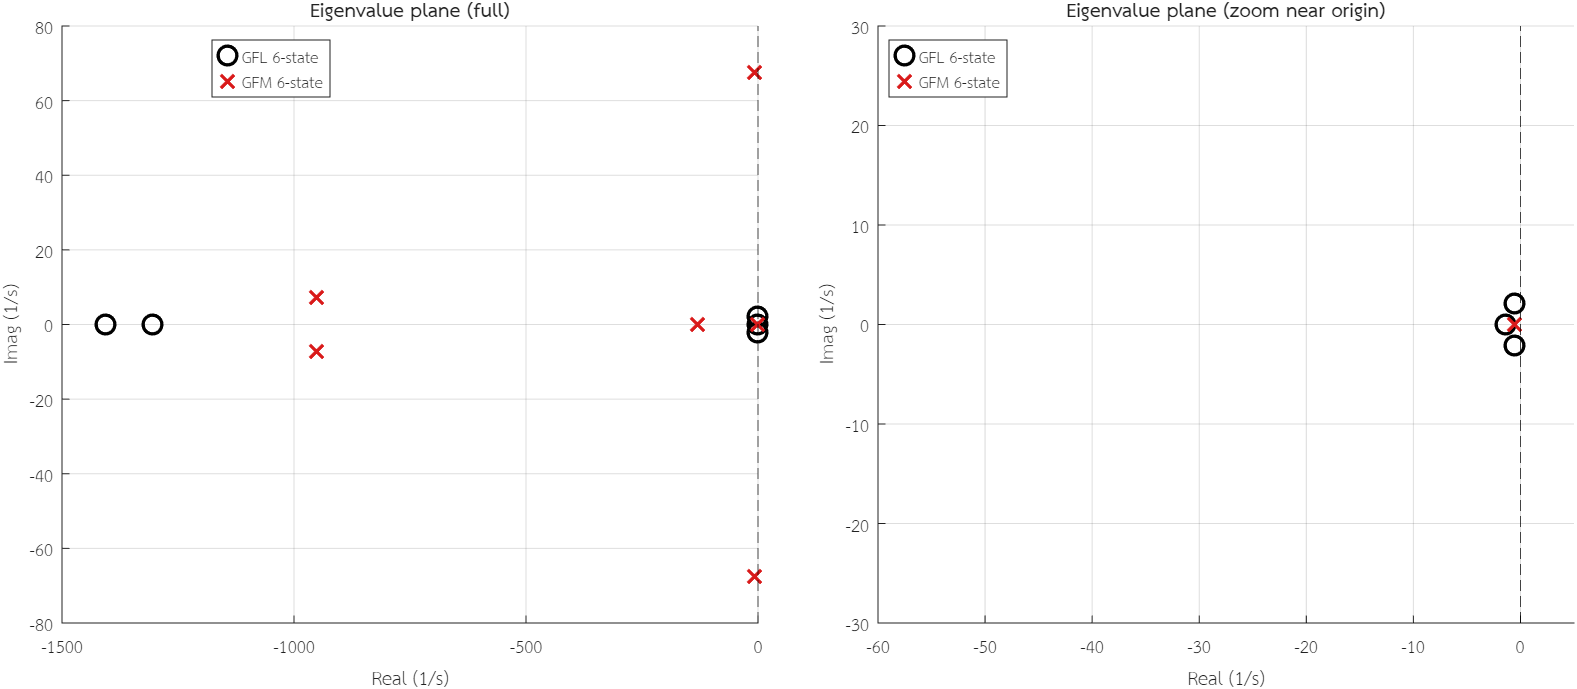
\includegraphics[width=\textwidth]{figures/ibr_gfl_gfm_th/eigenvalue_plane.png}
\caption{Eigenvalue บนระนาบเชิงซ้อน (ซ้าย: เต็ม, ขวา: ซูมใกล้จุดกำเนิด) วงกลมดำ = GFL 6-state,
กากบาทแดง = GFM 6-state ทุกโหมดอยู่ครึ่งซ้าย ($\Re<0$)}
\label{fig:eigplane}
\end{figure}

\subsection{ความถี่โมดัล (Hz)}

รูปที่~\ref{fig:modalfreq} แสดงความถี่ของโหมดเป็น Hz ซ้าย: ความถี่การสั่น $f=|\Im(\lambda)|/2\pi$ ของ
เฉพาะโหมดเชิงซ้อน (GFL swing PLL $\sim0.34$ Hz; GFM swing $\sim10.8$ Hz) ขวา: ความถี่ลักษณะ
$|\lambda|/2\pi$ ของทุกโหมด (สเกล log) แสดงการกระจายจากโหมดช้าไปโหมดเร็วของ current loop

\begin{figure}[H]\centering
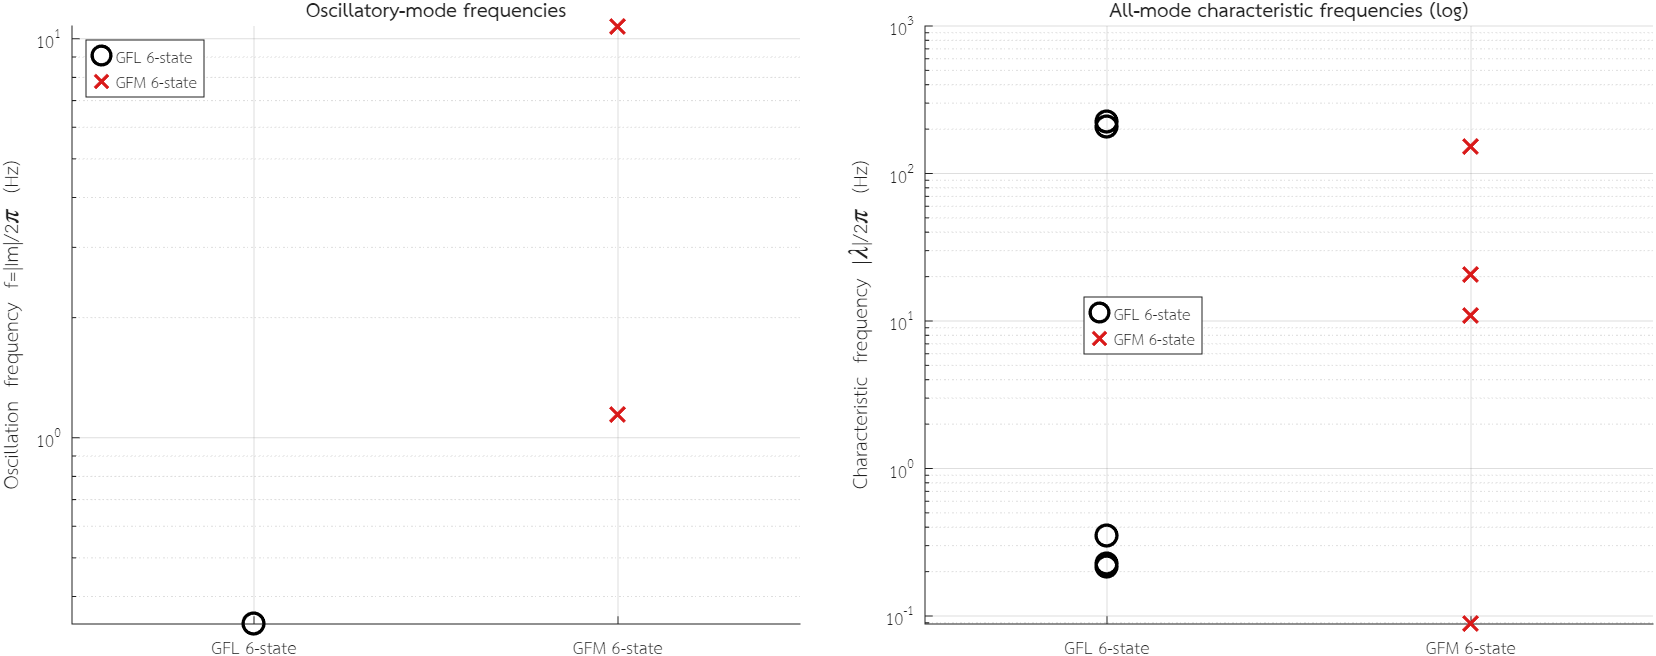
\includegraphics[width=\textwidth]{figures/ibr_gfl_gfm_th/modal_frequency.png}
\caption{ความถี่โมดัลเป็น Hz ซ้าย: ความถี่การสั่นของโหมดเชิงซ้อน; ขวา: ความถี่ลักษณะของทุกโหมด (log)}
\label{fig:modalfreq}
\end{figure}

\subsection{Eigenvalue เมื่อเพิ่มโหลด (+20\%, +40\%)}
\label{subsec:loadsweep}

เพื่อดูการเคลื่อนของ mode เมื่อ \emph{เพิ่มโหลด} (เพิ่ม $P_{ref}$ โดยคง $Q$) รูปที่~\ref{fig:eigloadsweep}
แสดง eigenvalue ที่ระดับโหลด \textbf{20\%, 40\%, 60\%, 80\%, 100\%} ($P=0.2,\,0.4,\,0.6,\,0.8,\,1.0$ pu)
ของทั้งสองแบบจำลอง (ซูมที่โหมดสั่นเด่นของแต่ละตัว) แต่ละระดับ re-solve equilibrium ใหม่แล้วคำนวณ SSSA ซ้ำ
ทุกระดับยังคง asymptotically stable โดย \emph{โหมด PLL ของ GFL แทบไม่ขยับ} ($0.34$ Hz คงที่) ขณะที่
\emph{โหมด swing ของ GFM ขยับชัด} (ความถี่ลดจาก $\sim10.9$ Hz ที่ 20\% เหลือ $\sim9.5$ Hz ที่ 100\%)

\begin{figure}[H]\centering
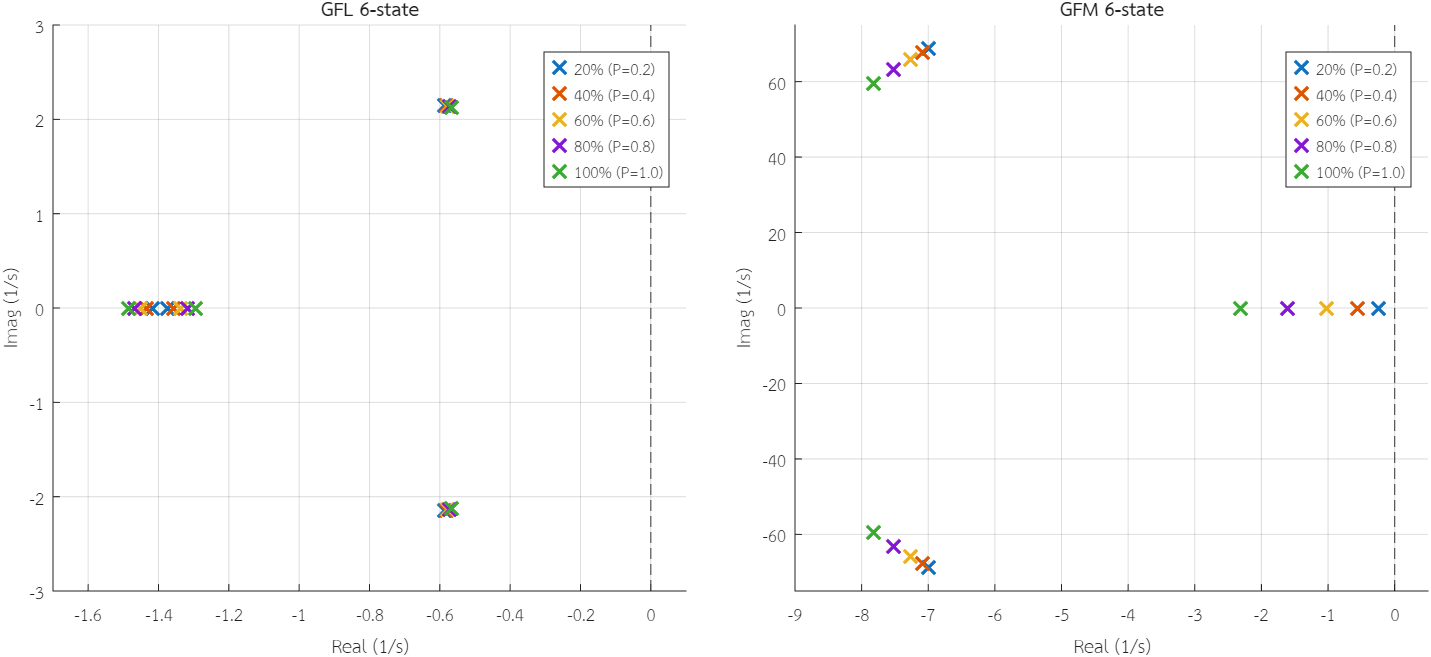
\includegraphics[width=\textwidth]{figures/ibr_gfl_gfm_th/eigenvalue_loadsweep.png}
\caption{Eigenvalue เมื่อกวาดโหลด 20/40/60/80/100\% ($P=0.2$--$1.0$ pu) ซ้าย: GFL 6-state (ซูมโหมด PLL
ใกล้จุดกำเนิด --- marker แทบทับกัน), ขวา: GFM 6-state (ซูมโหมด swing --- ขยับซ้าย/ความถี่ลดตามโหลด)
ทุกจุดยังอยู่ครึ่งซ้าย}
\label{fig:eigloadsweep}
\end{figure}

\subsection{ทำไมโหมด PLL ของ GFL แทบไม่ขยับ แต่โหมด swing ของ GFM ขยับตามโหลด}
\label{subsec:whymove}

eigenvalue คำนวณจากเมทริกซ์ $A$ ที่ linearise รอบ equilibrium เมื่อเพิ่ม $P_{ref}$ จุดทำงานใหม่
(มุมโหลด $\delta_0$, กระแส, แรงดันภายใน) เปลี่ยนไป \emph{เฉพาะช่องของ $A$ ที่เป็นฟังก์ชันไม่เชิงเส้นของ
จุดทำงานเท่านั้นที่จะเปลี่ยนค่า}

\paragraph{GFL --- โหมด PLL แทบไม่ขยับ.} วง PLL, PQ และ current ของ GFL ถูกกำหนดด้วย \emph{เกนคงที่}
(สมการ~\ref{eq:gfl-pll}) และแรงดันปลายทาง SMIB ที่แทบไม่เปลี่ยน (กริดแข็ง, คง $Q$) เมทริกซ์ $A$ จึงแทบ
ไม่ขึ้นกับ $P$ โหมด PLL ($-0.58\pm j2.14$) จึงเกือบนิ่ง marker ทับกันในรูป

\paragraph{GFM --- โหมด swing ขยับ.} สำหรับวง swing เมื่อ linearise จะได้
\begin{equation}
s^2+\underbrace{\frac{D_v}{M}}_{\text{หน่วง}}s+\underbrace{\frac{K_s\,\omega_b}{M}}_{\text{ความถี่}^2}=0,
\qquad K_s=\left.\frac{\partial P_e}{\partial\delta}\right|_0\ \propto\ \cos\delta_0,
\label{eq:swingchar}
\end{equation}
โดย $K_s$ คือสัมประสิทธิ์กำลังซิงโครไนซ์ ซึ่ง \emph{ขึ้นกับมุมโหลด} $\delta_0$ เมื่อเพิ่มโหลด $\delta_0$
โตขึ้น $\cos\delta_0$ ลดลง $K_s$ เปลี่ยน ทำให้ความถี่และตำแหน่งของโหมด swing \emph{ขยับเห็นได้} (ต่างจาก
GFL ที่ไม่มีมุมโหลดให้ขยับ) นี่คือความแตกต่างเชิงกายภาพหลักระหว่างการ \emph{ติดตาม} (GFL) กับการ
\emph{สร้าง} แรงดัน (GFM)

\section{การเปรียบเทียบ $i_d,i_q,P,Q$}

ตารางที่~\ref{tab:idqpq} แสดงค่า $i_d,i_q,P,Q$ ที่ equilibrium ทั้งสองแบบจำลอง settle ที่ $P=0.40$ pu,
$Q=0.10$ pu \emph{เท่ากัน} (จุดทำงานเดียวกัน) ค่า $i_d/i_q$ ต่างกันเพราะอยู่คนละกรอบอ้างอิง (GFL อิงมุม
$\delta_{PLL}$; GFM อิงมุมโรเตอร์ $\delta$) การเปรียบเทียบเชิงปริมาณจึงควรยึด $P,Q$ ที่เป็นค่าทางฟิสิกส์

\begin{table}[H]\centering\small
\caption{ค่า equilibrium $i_d,i_q,P,Q$ ของสองแบบจำลอง ($P,Q$ บน system base)}
\label{tab:idqpq}
\begin{tabular}{lcccccc}\toprule
Model & $n_x$ & $i_d$ (pu) & $i_q$ (pu) & $P$ (pu) & $Q$ (pu) & current frame\\\midrule
GFL 6-state & 6 & +0.4000 & -0.1000 & +0.4000 & +0.1000 & native\\
GFM 6-state & 6 & +0.3529 & -0.2132 & +0.4000 & +0.1000 & native\\
\bottomrule
\end{tabular}

\end{table}

การตอบสนองเชิงเวลาของ $i_d,i_q,P,Q$ ดูได้ \textbf{2 แบบ} ซึ่งให้ภาพต่างกันชัดเจน และเป็นประเด็นที่ควร
เข้าใจให้ถูก (ทั้งสองแบบใช้เมทริกซ์ $A$ ตัวเดียวกัน ความถี่การแกว่งจึงเท่ากันและตรงกับ eigenvalue)

\subsection{แบบ ก) รบกวนที่ $t=0$ (free small-signal ring-down)}
เนื่องจากไม่มี AVR/PSS จึง \textbf{ไม่มีเทอม $B\,\Delta u$} ($B=0$) ระบบเป็น autonomous
$\Delta\dot x = A\,\Delta x$ ในแบบนี้เรา \emph{ใส่การรบกวนไว้ที่เงื่อนไขเริ่มต้น} ($\Delta x_0$ เล็ก ๆ ที่
$t=0$) แล้ว integrate ด้วย \texttt{ode45} ผลคือกราฟ \textbf{แกว่งทันทีตั้งแต่ $t=0$ (ไม่มีช่วงแบน)}
เพราะระบบถูกดีดออกจาก equilibrium ตั้งแต่วินาทีแรก เป็นมุมมองไว้ดู \emph{โหมดธรรมชาติ/ความถี่} (GFM
แกว่ง swing $\sim10.8$ Hz, GFL แทบไม่แกว่ง) และเห็นว่าเมื่อเพิ่มโหลด 20--100\% ระดับ operating เลื่อนตาม

\begin{figure}[H]\centering
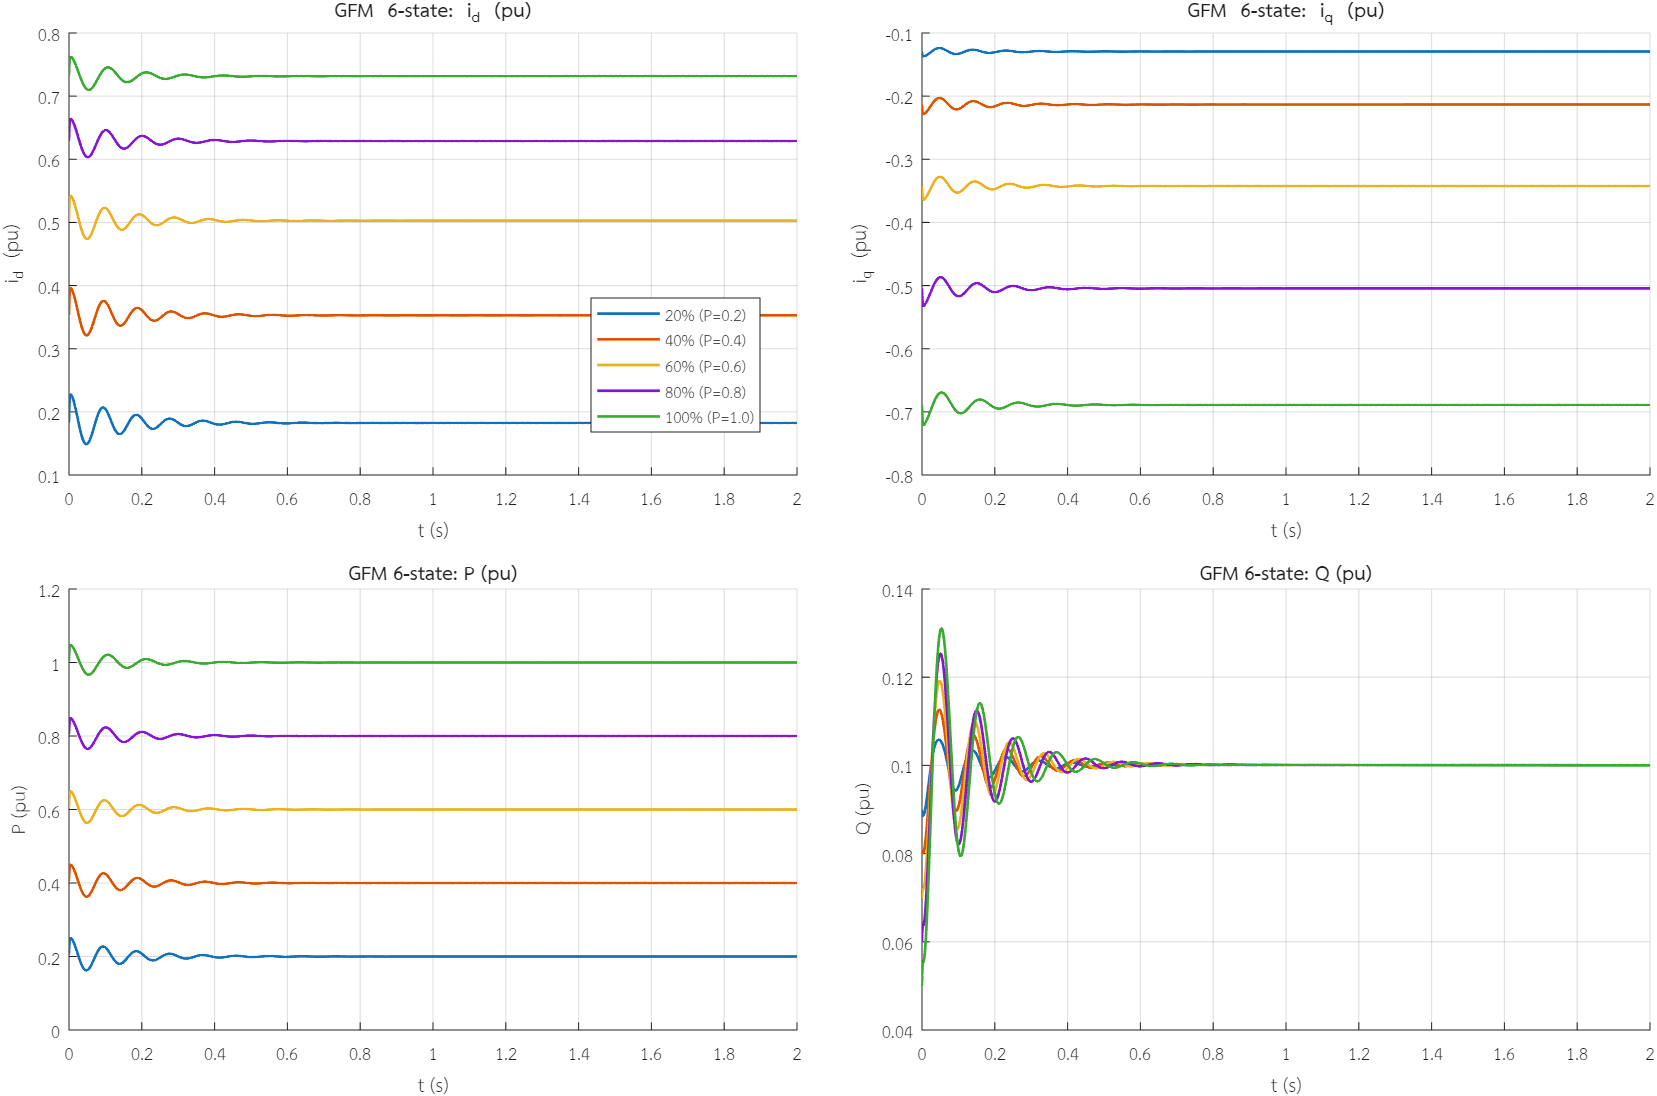
\includegraphics[width=\textwidth]{figures/ibr_gfl_gfm_th/pert_loads_gfm.png}
\caption{GFM 6-state --- free ring-down: ใส่ $\Delta x_0$ ที่ $t=0$ แล้ว integrate $\Delta\dot x=A\Delta x$
(\texttt{ode45}) ที่โหลด 20--100\% \emph{แกว่งตั้งแต่ $t=0$} (ไม่มีช่วงแบน)}
\label{fig:pertgfm}
\end{figure}

\subsection{แบบ ข) การตอบสนองต่อ fault (แบน $\to$ fault $\to$ ring-down)}
แบบนี้ \emph{เริ่มจาก equilibrium ที่ได้จาก PF พอดี} (static $=$ dynamic, $\|f_0\|\approx0$) แล้วใส่
\textbf{fault จริง} เป็น shunt impedance $Z_f$ ลงกราวด์ที่บัสช่วง $[t_{on},t_{clear}]$ (KCL:
$I_{dev}=(V-V_{inf})/Z_{line}+V/Z_f$) ผลคือกราฟ \textbf{แบนสนิทก่อน fault} (ไม่มี disturbance = ไม่แกว่ง)
แล้วจึงตอบสนองตอน fault และ ring-down กลับสู่ equilibrium หลังเคลียร์ --- นี่คือพฤติกรรมที่ถูกต้องของ
transient stability และเป็นคำตอบต่อข้อสังเกตที่ว่า ``ถ้าไม่มี fault ก็ไม่ควรแกว่ง'' (เหมือน SG)

\begin{figure}[H]\centering
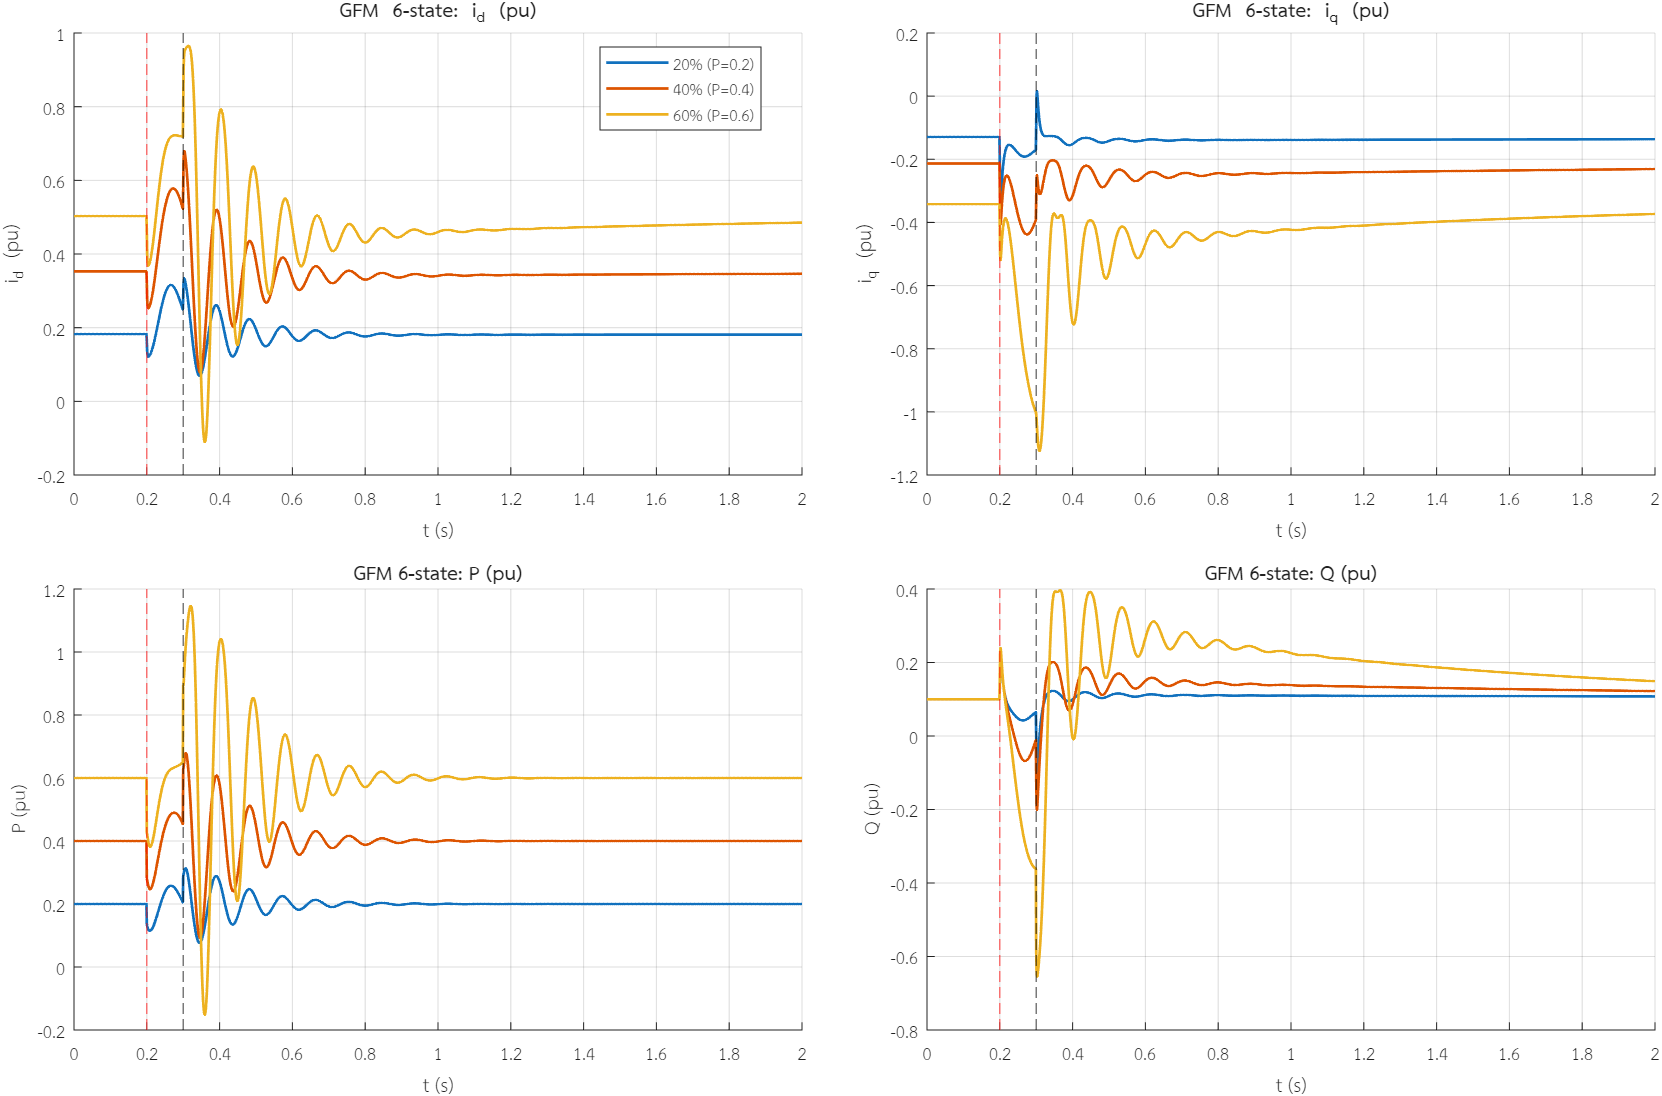
\includegraphics[width=\textwidth]{figures/ibr_gfl_gfm_th/ode45_loads_gfm.png}
\caption{GFM 6-state --- fault response ($Z_f=0.5j$ pu, $0.2$--$0.3$ s) ที่โหลด 20/40/60\%
\emph{แบนก่อน fault} (เส้นแดง = fault on, เส้นดำ = clear) แล้ว ring-down กลับ equilibrium}
\label{fig:ode45gfm}
\end{figure}

\begin{figure}[H]\centering
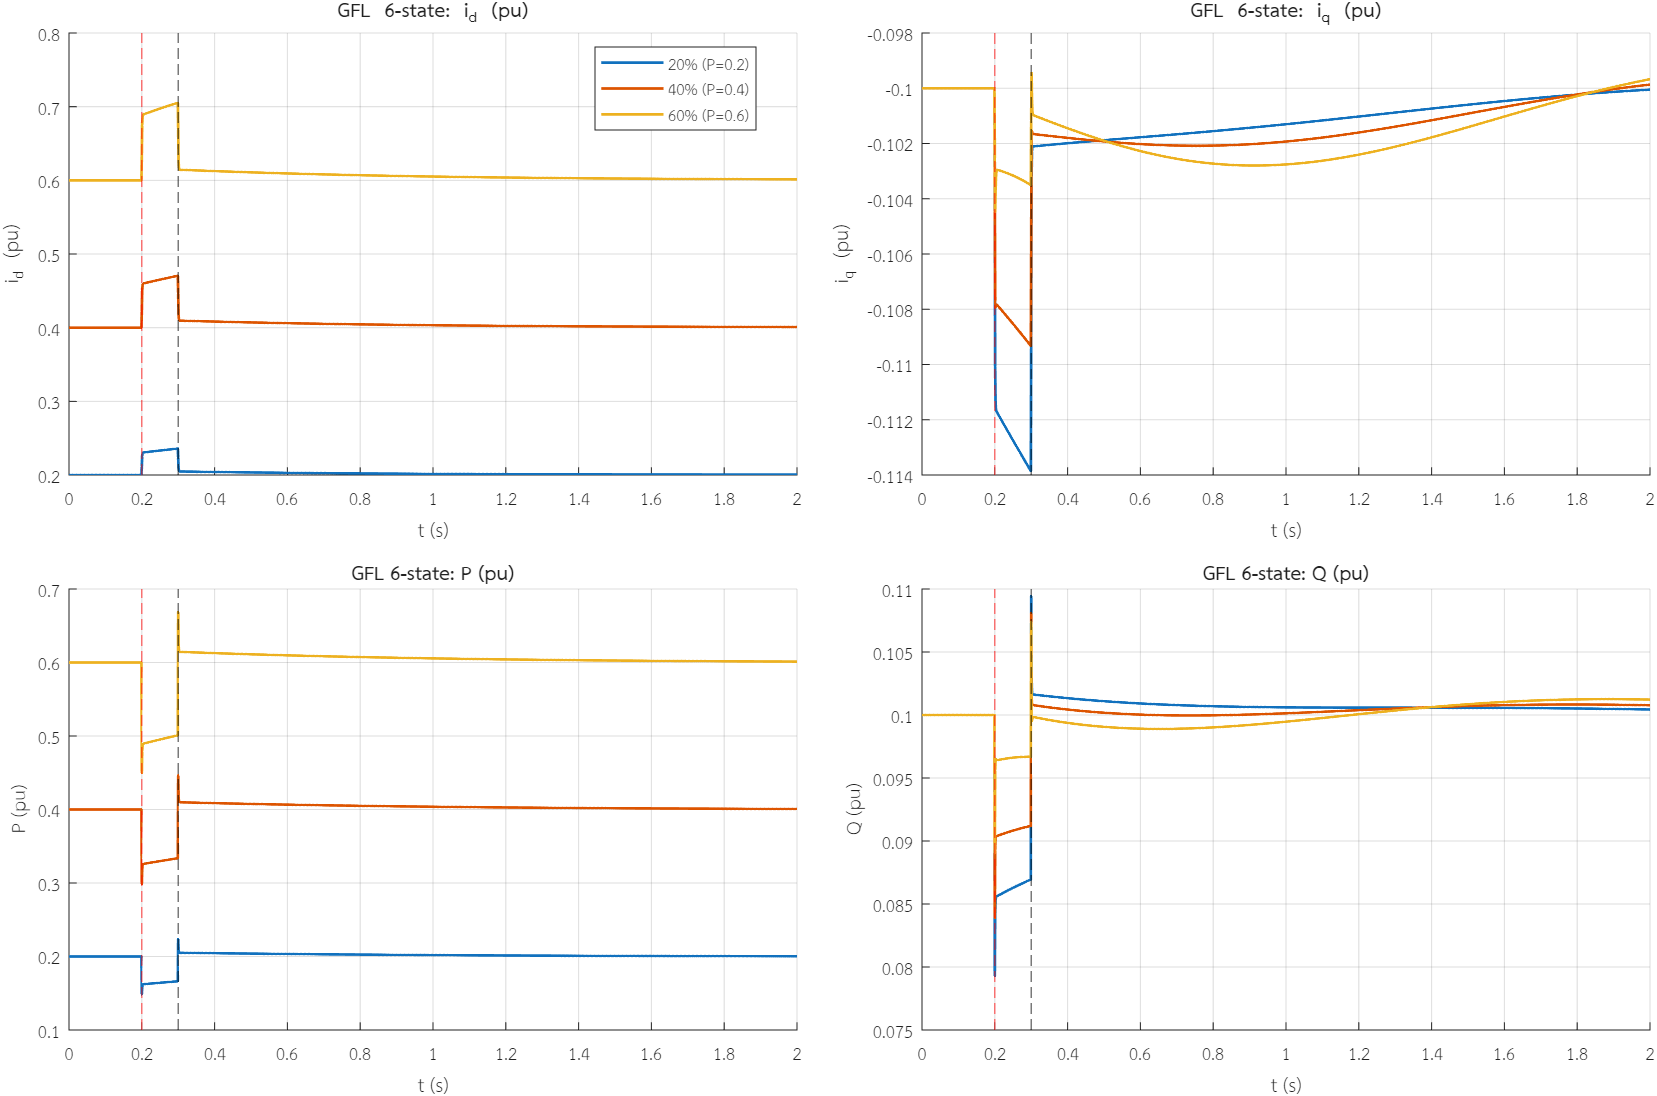
\includegraphics[width=\textwidth]{figures/ibr_gfl_gfm_th/ode45_loads_gfl.png}
\caption{GFL 6-state --- fault response ($Z_f=0.5j$ pu, $0.2$--$0.3$ s) ที่โหลด 20/40/60\%
แบนก่อน fault แล้วตอบสนอง (โหมด PLL ช้า จึงหน่วงเรียบกว่า GFM)}
\label{fig:ode45gfl}
\end{figure}

\noindent\textbf{ความถี่ระหว่าง fault.} รูปที่~\ref{fig:freq} เทียบความถี่ของสองแบบจำลอง: ฝั่ง GFL คือ
\emph{ความถี่ที่ PLL ประมาณได้} ($f=f_{base}+(k_{p,PLL}v_q+k_{i,PLL}\xi_{PLL})/2\pi$) ส่วน GFM คือ
\emph{ความถี่โรเตอร์เสมือน} ($f=f_{base}\cdot\omega$) ทั้งคู่ \textbf{แบน 60 Hz ก่อน fault} จากนั้น:
GFL เบี่ยงความถี่ \emph{น้อยมาก} ($\sim\pm0.01$ Hz --- เพราะ PLL เพียง ``ติดตาม'' มุมกริด) ขณะที่ GFM
เบี่ยง \emph{มาก} (แกว่ง $\sim51$--$66$ Hz ที่โหลด 60\%) แล้วหน่วงกลับ 60 Hz --- นี่คือ \emph{inertia
response} ของ virtual rotor ที่มีความเฉื่อยต่ำ ($M=0.08$ s) ซึ่งเป็นบริการเสริมความถี่ที่ GFM ให้แต่ GFL ไม่ให้

\begin{figure}[H]\centering
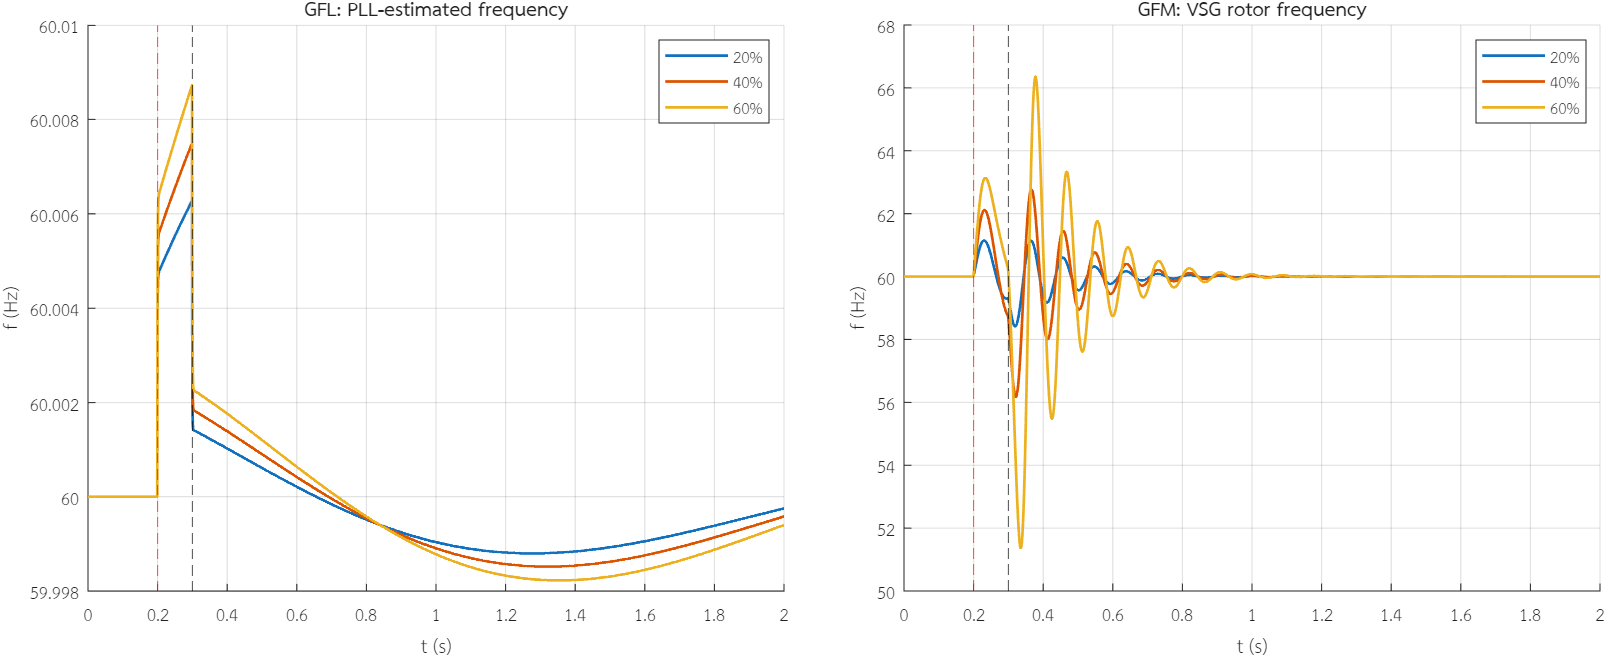
\includegraphics[width=\textwidth]{figures/ibr_gfl_gfm_th/freq_loads.png}
\caption{ความถี่ $f$ (Hz) ระหว่าง fault ที่โหลด 20/40/60\% ซ้าย: GFL --- ความถี่ที่ PLL ประมาณ (เบี่ยงน้อย,
ติดตามกริด); ขวา: GFM --- ความถี่โรเตอร์ VSG (แกว่งมากแล้วหน่วง, inertia response) ทั้งคู่แบน 60 Hz ก่อน fault}
\label{fig:freq}
\end{figure}

\noindent สุดท้าย รูปที่~\ref{fig:combined} รวม \emph{ทุกปริมาณในภาพเดียว} (จำลอง 15 วินาที): ความถี่ (แกน Y
สองข้าง) พร้อม $i_d,i_q,P,Q$ ของ GFL (ส้ม-ประ) เทียบ GFM (น้ำเงิน-ทึบ) หลัง grid step เดียวกัน เห็นภาพรวม
ครบ: GFM ตอบสนองเร็ว/แกว่งกว้าง (มีความเฉื่อย, สร้างแรงดัน) ส่วน GFL ช้า/เบา (ติดตามกริด) โดยทั้ง $P$ กลับสู่
$P_{ref}=0.4$ และ $Q$ ของ GFM ยกขึ้นหนุนแรงดันหลัง step

\begin{figure}[H]\centering
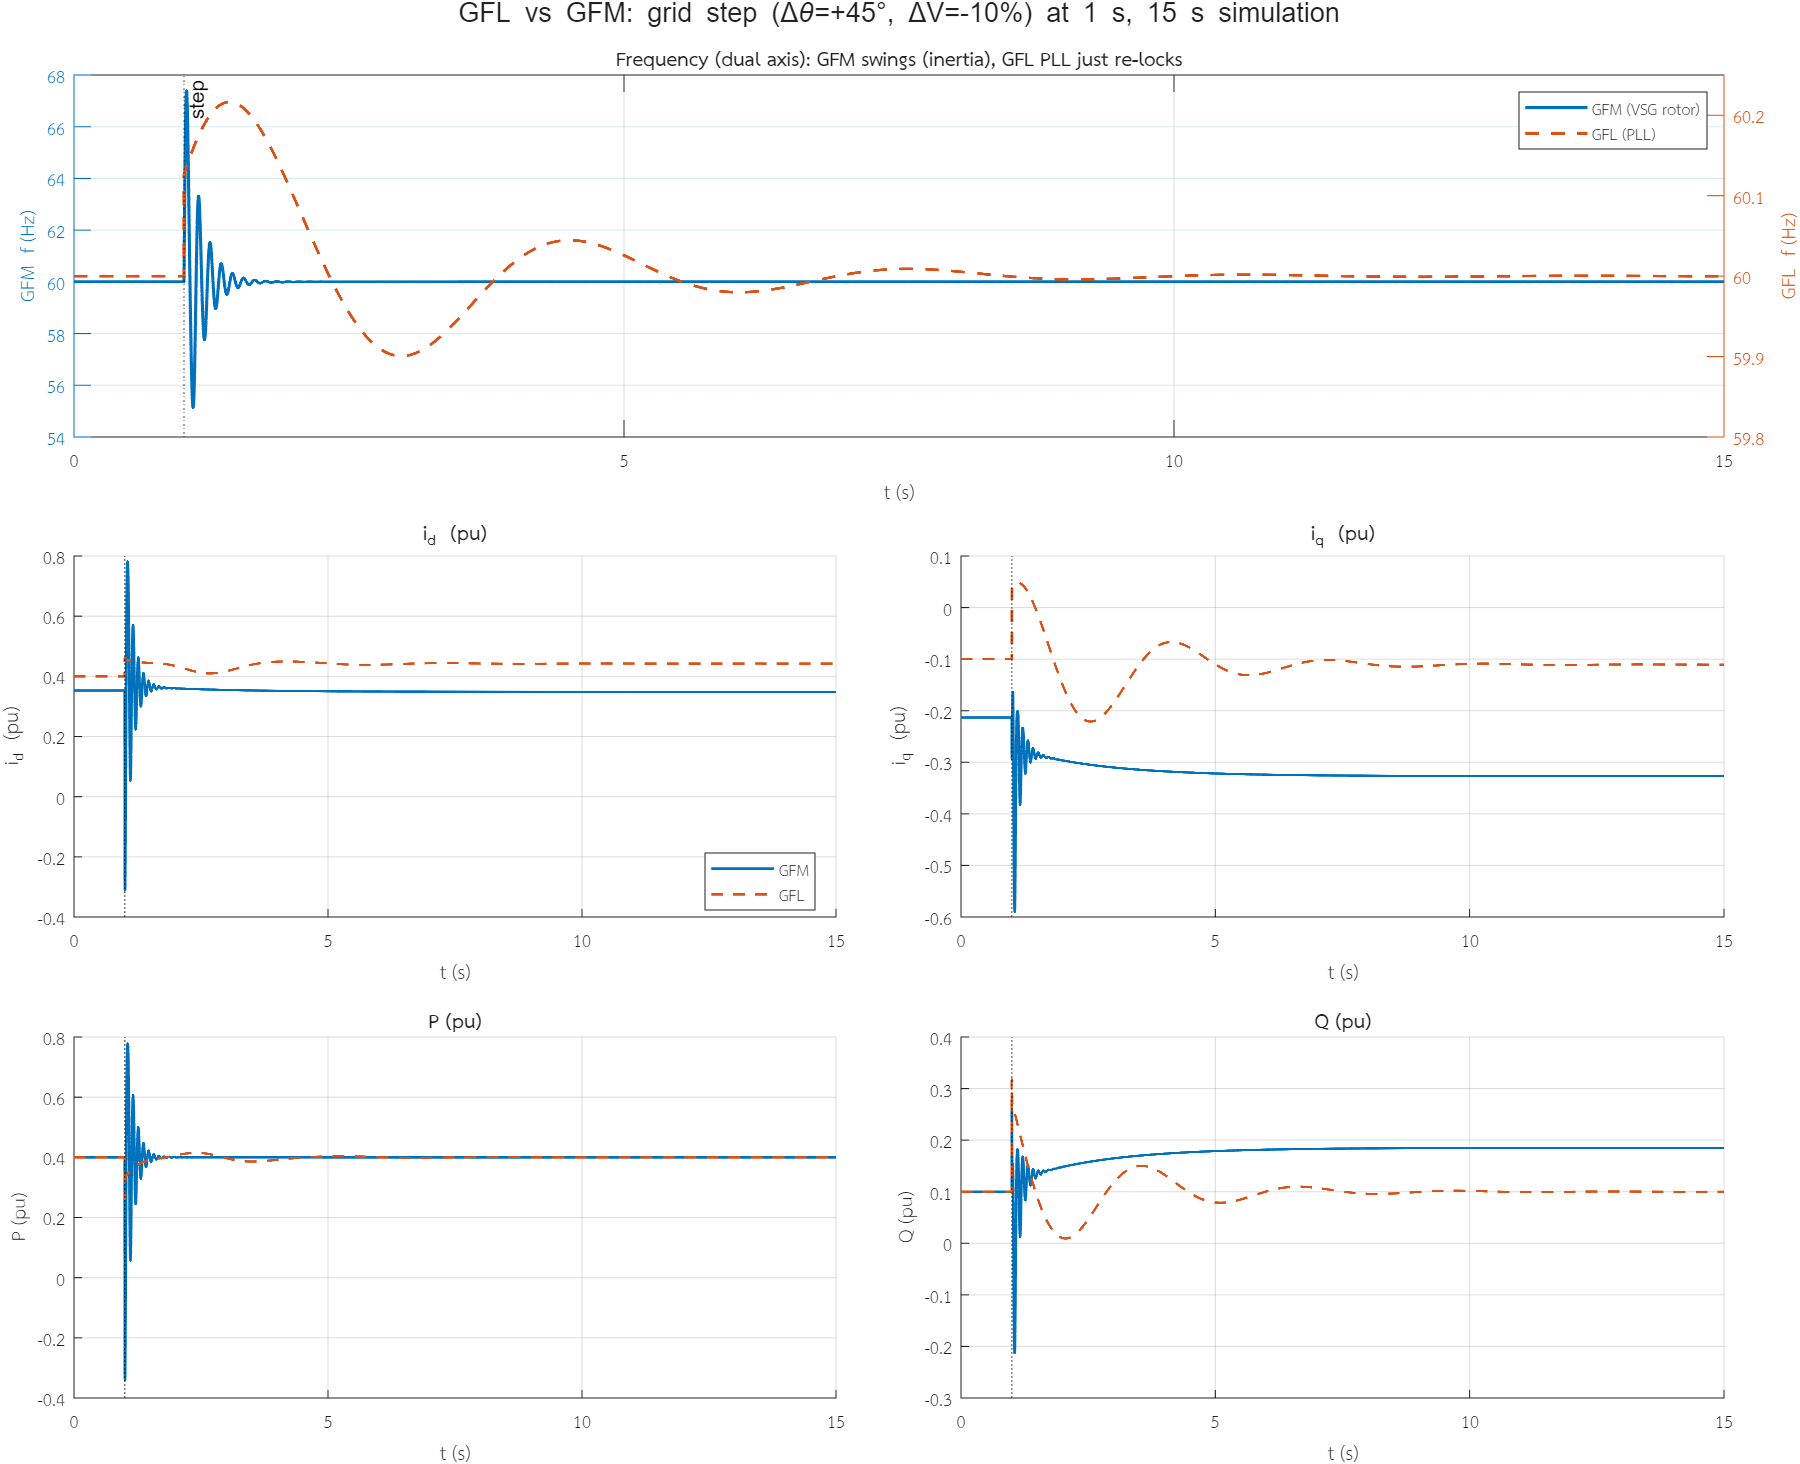
\includegraphics[width=\textwidth]{figures/ibr_gfl_gfm_th/combined_step.png}
\caption{ภาพรวมในรูปเดียว: ความถี่ (แกนคู่) + $i_d,i_q,P,Q$ ของ GFL vs GFM หลัง grid step
($\Delta\theta=+45^\circ$, $\Delta V=-10\%$) ที่ 1 วินาที จำลอง 15 วินาที (GFM น้ำเงินทึบ, GFL ส้มประ)}
\label{fig:combined}
\end{figure}

\subsection{เปรียบเทียบและข้อสรุป}
ความต่างของสองภาพ \textbf{ไม่ได้อยู่ที่ตัวแบบจำลอง} (ใช้ $A$ เดียวกัน) แต่อยู่ที่ \emph{ตำแหน่งของการรบกวน}:
\begin{itemize}\itemsep2pt
  \item แบบ ก) ใส่การรบกวนที่ \emph{เงื่อนไขเริ่มต้น} ($t=0$) $\Rightarrow$ แกว่งทันที ไม่มีช่วงแบน
  (มุมมองโหมดธรรมชาติ; ใช้เทียบกับ eigenvalue/$f,\zeta$ ได้โดยตรง)
  \item แบบ ข) เริ่มที่ equilibrium แล้วใส่การรบกวน (fault) ที่ \emph{เวลาหนึ่งภายหลัง} $\Rightarrow$
  \emph{แบนก่อน} แล้วจึงแกว่งหลัง fault (มุมมอง transient stability ที่ถูกต้อง)
\end{itemize}
ประเด็นสำคัญคือ \textbf{โมเดลเรา static $=$ dynamic แล้ว} ($\|f_0\|\approx0$, event-free drift $=0$) ดังนั้น
\emph{ถ้าไม่ใส่ fault กราฟจะแบนสนิท ไม่แกว่งเอง} เช่นเดียวกับ SG การที่ IBR ``แกว่ง'' ในแบบ ก) เป็นเพราะ
เราจงใจดีดมันออกจาก equilibrium ที่ $t=0$ ไม่ใช่เพราะ static $\neq$ dynamic การแกว่งหลัง fault ในแบบ ข)
คือฟิสิกส์จริง (โหมด swing/PLL) ซึ่งทั้ง SG และ IBR ต่างก็แกว่งเมื่อเจอ fault

\noindent\emph{หมายเหตุ (ขีดจำกัด transient stability):} แบบ ข) แสดงโหลด 20/40/60\% เพราะที่โหลดสูงกว่า
($\gtrsim70\%$) มุมโหลด $\delta_0$ ใหญ่จน margin ซิงโครไนซ์เหลือน้อย เมื่อเจอ fault เดียวกัน GFM แบบลดรูป
(\emph{ไม่มี} current limiter/LVRT) จะ \emph{สูญเสีย synchronism} หลังเคลียร์ ซึ่งเป็นขีดจำกัด transient
stability จริงของแบบจำลองศึกษานี้ (การเพิ่ม current limiter/LVRT เป็นงานต่อยอด)

\section{สรุป}

รายงานนี้นำเสนอแบบจำลอง IBR แบบลดรูป 6 states สองชุด (GFL และ GFM) ที่จัดโครงสร้างเป็น 3 บล็อก บล็อกละ 2
states ตามงาน EECON49 ทั้งสองผ่านการตรวจ equilibrium (residual ระดับ machine precision) และ SSSA พบว่า
\emph{เสถียรทุกโหมด} และ \emph{มีโหมดสั่น (complex)} ตามที่คาดในทฤษฎี: GFL มีโหมด PLL ($\sim0.34$ Hz) และ
GFM มีโหมด swing ($\sim10.8$ Hz) เมื่อเพิ่มโหลด โหมด PLL ของ GFL แทบไม่ขยับ (เกนคงที่) ขณะที่โหมด swing
ของ GFM ขยับตามสัมประสิทธิ์ซิงโครไนซ์ $K_s\propto\cos\delta_0$ ซึ่งสะท้อนความแตกต่างเชิงกายภาพระหว่างการ
ติดตามและการสร้างแรงดัน

\begin{thebibliography}{9}
\bibitem{yazdani2010} A.~Yazdani and R.~Iravani, \emph{Voltage-Sourced Converters
in Power Systems: Modeling, Control, and Applications}. Hoboken, NJ: Wiley/IEEE
Press, 2010.
\bibitem{teodorescu2011} R.~Teodorescu, M.~Liserre, and P.~Rodr\'iguez,
\emph{Grid Converters for Photovoltaic and Wind Power Systems}. Chichester, UK:
Wiley/IEEE Press, 2011.
\bibitem{bacha2014} S.~Bacha, I.~Munteanu, and A.~I.~Bratcu, \emph{Power
Electronic Converters Modeling and Control}. London: Springer, 2014.
\bibitem{sakimoto2015} K.~Sakimoto, Y.~Miura, and T.~Ise, ``Virtual Synchronous
Generator without Phase Locked Loop based on Current Controlled Inverter and its
Parameter Design,'' \emph{IEEJ Trans.\ Power and Energy}, vol.~135, no.~7,
pp.~462--470, 2015.
\bibitem{pogaku2007} N.~Pogaku, M.~Prodanovi\'c, and T.~C.~Green, ``Modeling,
Analysis and Testing of Autonomous Operation of an Inverter-Based Microgrid,''
\emph{IEEE Trans.\ Power Electronics}, vol.~22, no.~2, pp.~613--625, 2007.
\bibitem{eecon49} P.~Jueajan, P.~Phadungdaen, S.~Jaingeawkham, T.~Surinkaew, and
I.~Ngamroo, ``A Bayesian Optimization-Based GFL/GFM Mode Switching Strategy for
Dynamic Stability Enhancement in Low-Inertia Power Systems,'' EECON49 (submitted),
KMITL, 2026.
\end{thebibliography}

\end{document}
